% $Id: conclusion.tex 
% !TEX root = main.tex

%%
\section{\ac{RL} Agents with Adaptive Behavior}
\label{sec:implementation}

This section introduces \adaptiverl, our proposed approach for enabling \ac{RL} agents to 
dynamically adapt their behavior in response to evolving environmental conditions, specifically 
changes in the goal state and available agent actions. Our method enables agents to 
pursue shifting objectives throughout their operational lifespan and acquire new capabilities as 
tasks change over time. \adaptiverl is made of two main parts:
\begin{enumerate*}[label=(\arabic*)]
\item monitoring the environment for changes,
\item adapting agents' behavior to new goals and incorporating new actions.
\end{enumerate*}
The implementation of our work is publicly available.\footnote{Available at: \url{https://anonymous.4open.science/r/morphin_rl}}

The conceptual foundation of \adaptiverl aligns with the ideas proposed 
by~\citet{abel2023definitioncontinualreinforcementlearning} for \ac{CRL}, emphasizing continual 
adaptation rather than convergence to a fixed solution. We extend tabular Q-learning by integrating 
adaptive mechanisms that enable agents to dynamically adjust their learning strategies in response 
to detected environmental changes. Similar to the approach described 
by~\citet{norman2024firstexploreexploitmetalearningsolve}, every time a change is detected, be that 
a significant change in the rewards or the introduction of new actions, our agent thoroughly explores 
the environment while retaining information of previously learned policies. The exploration process 
continues until a new policy stabilizes, to then exploit the acquired knowledge. Applying such 
strategy agents can rapidly convergence to new environment configurations, without entirely 
discarding previously learned knowledge.

To enable agents to adapt their behavior to new conditions, we introduce an adaptive mechanisms 
that adjust the agent's learning rate (\lrate{\alpha}) and exploration rate ($\varepsilon$) in conjunction 
with a concept drift detection strategy. By continuously monitoring and responding to changes in the 
environment, agents can autonomously modify their learning process at run time, enabling them 
to learn new behavior to attain their goals, even if these change. This capability positions our 
approach within the class of self-adaptive systems (SAS)~\cite{sasreview}, ensuring continual 
adaptation and resilience in non-stationary contexts.

%%%%
\subsection{Environment monitoring and drift detection}

The first step for agents to adapt their behavior to an evolving environment is to continuously monitor 
the environment. \ac{RL} environment monitoring is intrinsic through the interaction with the 
environment, as agents continuously observed rewards after each action execution. To detect 
changes in the environment, \ie drift, we implement the 
PH-test~\cite{mignon2017adaptive,networkdynamicrl}. The PH-test calculates the cumulative 
difference between observed rewards and the running mean reward, incorporating a sensitivity 
parameter ($\delta$). A concept drift (environmental change) is flagged when the cumulative 
difference surpasses a predefined threshold. Selecting an appropriate threshold value is crucial, as it 
determines the sensitivity of drift detection. Higher thresholds result in more conservative detection, 
while lower thresholds increase sensitivity to changes, this value must be selected based on the 
magnitude order of rewards and posible changes over them.

Building on the concept of drift detection, and following the ideas of~\citet{mignon2017adaptive}, 
we adaptively increase the exploration rate ($\varepsilon$) whenever the PH-test detects a concept 
drift. This approach promotes exploration immediately following environmental changes, enabling 
the agent to acquire new knowledge by temporarily adopting an exploration-focused policy. To 
ensure adequate exploration, the agent maintains an elevated exploration rate until rewards 
stabilize (\ie the cumulative difference is below the threshold, and  no further drifts are detected). 
Once stable, the exploration rate $\varepsilon$ uses a decay policy, leading the agent to exploit its 
behavior.

This adaptive drift detection mechanism ensures the agent maintains an effective balance between 
exploring new environment dynamics and leveraging previously acquired knowledge. It is crucial to 
ensure a high exploration rate after concept drift is detected consistently, so the agent can learn a 
new policy (\ie behavior) without forgetting previously acquired knowledge. \fref{fig:dynamic-eps}, 
shows the behavior of the dynamic exploration rate ($\varepsilon^*$) in our non-stationary Gridworld 
running example.

\begin{figure*}[hptb]
    \centering
    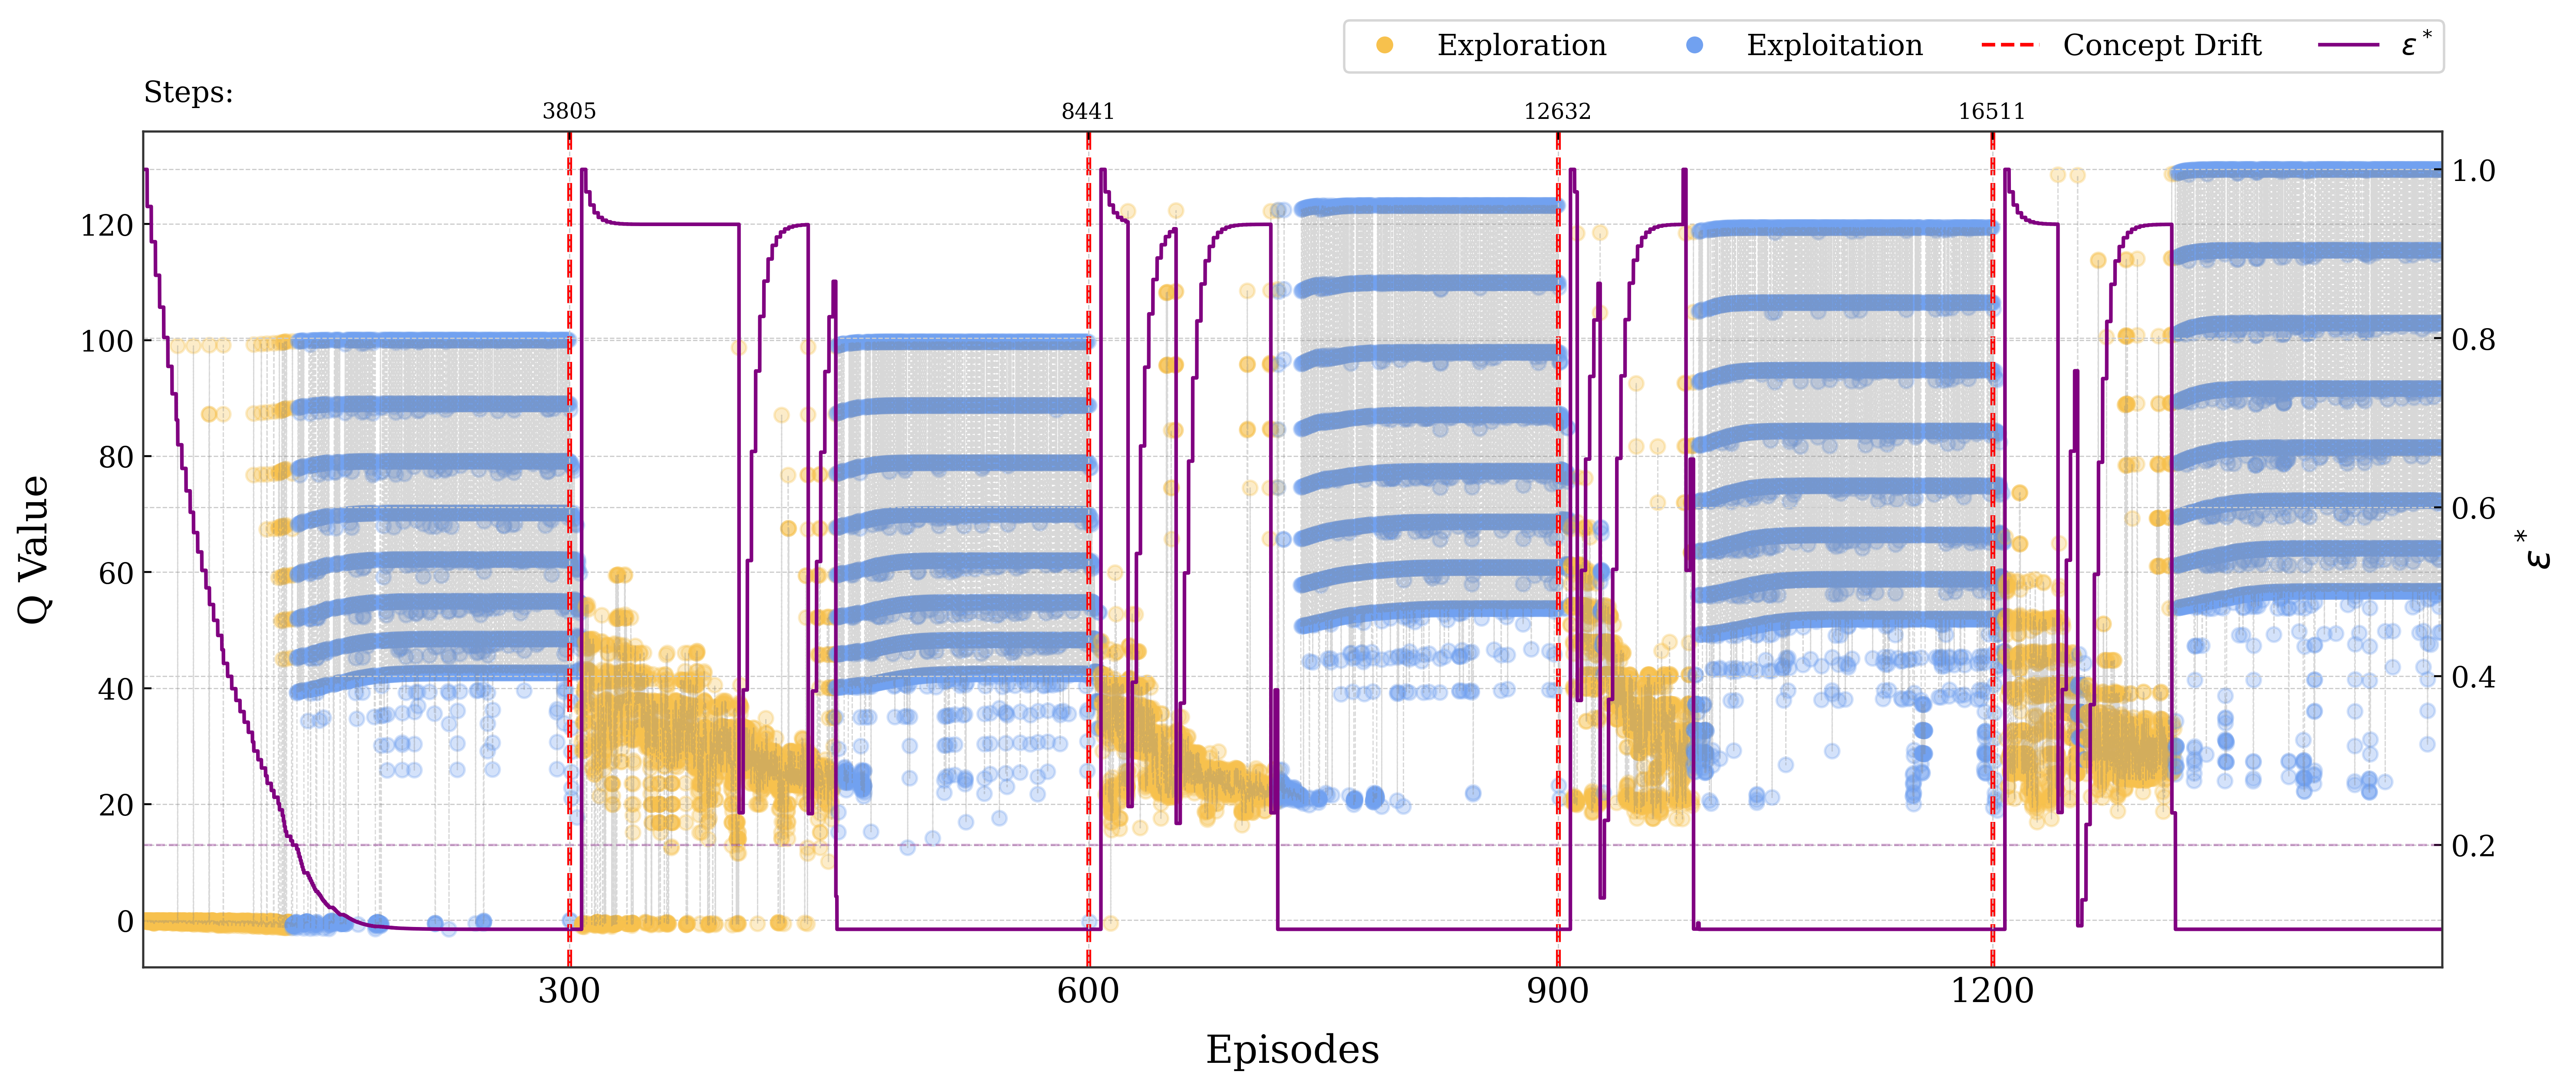
\includegraphics[width=\textwidth]{figures/eps}
    \caption{\adaptiverl's adaptive behavior of the dynamic exploration rate ($\varepsilon^*$) in Non-Stationary Gridworld experiments. Observe how $\varepsilon^*$ increases whenever a concept drift is detected by the PH-test and remains elevated until the agent consistently achieves the expected rewards (i.e., no further drift and stable rewards). Once stability is reached, $\varepsilon^*$ decays toward its minimum value, allowing the agent to exploit the acquired knowledge.}
    \label{fig:dynamic-eps}
\end{figure*}

%%%%
\subsection{Adaptation to Changing Goals and new Actions}
\label{sec:morphin-adaptation}

The key to enable agents is to, on the one hand, keeping knowledge gained under previous 
environment conditions, and to dynamically adjusting the learning rate (\lrate{\alpha}) in response 
to detected drift. The learning rate is modified dynamically using the Temporal Difference (TD) error 
defined in \fref{eq:td_error}.

\begin{equation} \label{eq:td_error}
    TD_{error} = r_{t+1} + \gamma \cdot \underset{a}{\max} Q(s_{t+1}, a) - Q(s_t, a_t)
\end{equation}

The TD error quantifies the difference between the agent's predicted reward and the actual reward 
received. The dynamic learning rate (\lrate{\alpha^*}) is then adjusted based on the TD error 
following \fref{eq:dynamic_learning_rate}.

\begin{equation}
    \label{eq:dynamic_learning_rate}
    \alpha^* = \alpha + (\alpha_{\max}-\alpha) \cdot \frac{1}{1 + e^{-(|TD_{error}|-k)}}
\end{equation}

In the equation, \lrate{\alpha} corresponds to the base learning rate (e.g., 0.1), and $\alpha_{\max}$ 
is the upper bound of the learning rate (\eg 0.9 specified during the creation of the agent). This 
method introduces a new learning parameter $k$, which controls the sensitivity of the learning rate to 
the TD error, with higher values resulting in reduced sensitivity. Parameter $k$ must be carefully (and 
empirically) tuned according to the specific characteristics of the environment and learning context. 
High TD errors induce a larger learning rate, enabling faster updates during exploration, whereas 
lower TD errors yield a more stable and conservative learning process during exploitation phases. 
\fref{fig:alpha} illustrates the behavior of the dynamic learning rate (\lrate{\alpha^*}). In the figure it 
is possible to observe that the agent is able to detect the concept drift and enable exploration short 
after the drift occurs. Moreover, after the second concept drift, the exploration period of the agent 
shortens. This is due fact that agents do not loose their knowledge after a concept drift is detected. 
As a consequence, agents take more informed decisions after every episode, leading to higher 
rewards. 

\begin{figure*}[hptb]
    \centering
    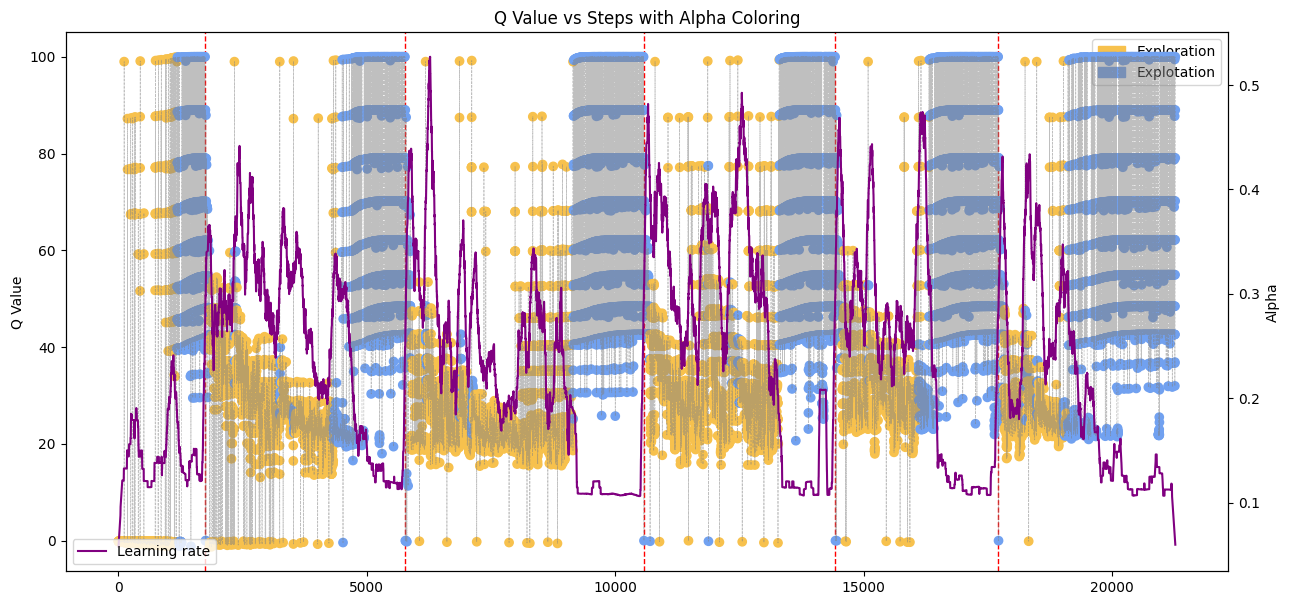
\includegraphics[width=\textwidth]{figures/alpha}
    \caption{\adaptiverl's adaptive behavior of the dynamic learning rate ($\alpha^*$) in Non-Stationary Gridworld experiments. Notice how $\alpha^*$ increases during exploration phases (when the TD error is high) and decreases during exploitation phases (when the TD error is low), enabling rapid convergence during exploration and stable learning during exploitation.}
    \label{fig:alpha}
\end{figure*}

The adaptation in the case of the introduction of new actions to an agent, follows the same process 
as the adaptation to changing goals. Agents can be given new capabilities with the introduction of 
actions as a direct signal to the agent, in which case the dynamic adaptation process is triggered 
instantly to enable the exploration taking into account the new action. Another possibility is that the 
action is obtained unannounced, in which case the agent can detect the new action during the 
monitoring, and then use the dynamic learning rate.

Whichever method used, agents using the dynamic learning rate strategy, agents explore the 
environment anew, enabling the discovery of new or improved behavior due to the acquired actions. 
The overall performance of the agent improves or keeps the same, as the goals remain unchanged.

Finally note that if both the goals change, and the agent acquires new actions simultaneously, 
The proposed strategy can detect both situations as concept drift, and trigger the learning process 
to effectively resolve the two variation points.


\endinput

